\chapter{\xlabel{pol2_dr}POL-2 Data Reduction - Running pol2map}
\label{sec:rundr}

The previous chapter, \cref{Chapter}{sec:dr}{POL-2 Data Reduction - The Theory}, described how pol2 map produces I Q and U maps from raw POL-2 data. 
It showed that this reduction process - which uses pol2map - is a three step process.  

As with the other Python scripts in SMURF, you can get more information about the available
parameters by doing either:
\begin{terminalv}
% pol2map --help
\end{terminalv}
or
\begin{terminalv}
% smurfhelp pol2map
\end{terminalv}

\section{\xlabel{how-pol2map}How to use pol2map}

Before running pol2map directly, you need to ensure that the \starlink\ environment has been 
initialised and the \smurf\ package started (see
\cref{Section}{sec:starinit}{Initialising Starlink} and
\cref{Section}{sec:packinit}{KAPPA and SMURF for data processing}).
To run pol2map you need to supply values for the 
following command-line parameters\footnote{Note the distinction between
``command-line parameters'' (also known as ``ADAM'' parameters) that are
supplied on the \texttt{makemap} command line, and ``configuration parameters''
that are specified within a configuration file. Values for all
\emph{configuration} parameters are obtained using a single \emph{command-line}
parameter called \texttt{CONFIG}.}:



\begin{aligndesc}
\item[\texttt{IN}] A list of input NDFs containing raw POL-2 data. 
There are many ways in which the list of files can be supplied,
as described in Section ``\xref{Specifying Groups of Objects}{sun95}{se_groups}''
in \xref{SUN/95}{sun95}{}. The easiest is to create a simple text
file containing the names of the raw data files -- one per line --- and
then supply the name of the text file, preceded by an up-caret character
(\,\texttt{\^{}}\,), as the value for parameter \texttt{IN}. Note, the names of
the raw data files can contain wild-cards such as ``$*$'' and ``?''.

\item[\texttt{IOUT}] 
The name of the NDF in which to store the the total intensity (I) map
including all supplied observations. The supplied file name should either have a file type of
``\texttt{.sdf}'', or no file type at all (in which case \texttt{.sdf}
will be appended to the supplied value). Any existing file with the same
name will be over-written.

\item[\texttt{QOUT}] 
The output NDF in which to return the Q map including all supplied
observations. This will be in units of pW. Supply null (!) if no Q
map is required.


\item[\texttt{UOUT}] 
The output NDF in which to return the U map including all supplied
observations. This will be in units of pW. Supply null (!) if no U
map is required.

\item[\texttt{MAPDIR}] 
The name of a directory in which to put the Q, U an I maps made
from each individual observation supplied via "IN", before
coadding them. If
null is supplied, the new maps are placed in the same temporary
directory as all the other intermediate files and so will be
deleted when the script exists (unless parameter RETAIN is set
TRUE). Note, these maps are always in units of pW. Each one will
contain FITS headers specifying the pointing corrections needed
to align the map with the reference map. [!]


\item[\texttt{QUDIR}] 
The name of a directory in which to put the Q, U and I time series
generated by SMURF:CALCQU, prior to generating maps from them. If
null (!) is supplied, they are placed in the same temporary directory
as all the other intermediate files and so will be deleted when the
script exists (unless parameter RETAIN is set TRUE). [!]


\end{aligndesc}

\section{\xlabel{how-step1}pol2map - producing the initial I map.}

As discussed in \cref{Chapter}{sec:dr}{POL-2 Data Reduction - The Theory} we must first run pol2map on the raw data to produce an initial I map.

In this first step we run:

\begin{terminalv}
% pol2map in=^myfiles.list iout=iauto qout=! uout=! mapdir=maps qudir=qudata
\end{terminalv}


Here, the file \texttt{myfiles.lis} contains a list of the raw data
files to be included in the map, and could for instance look like this:

\begin{terminalv}
% cat myfiles.lis
/jcmtdata/raw/scuba2/s8a/20160125/00043/*
/jcmtdata/raw/scuba2/s8b/20160125/00043/*
/jcmtdata/raw/scuba2/s8c/20160125/00043/*
/jcmtdata/raw/scuba2/s8d/20160125/00043/*
\end{terminalv}

This uses all available data for all four 850\,$\mu$m sub-arrays, for
observation 43 taken on 25th January 2016\footnote{The input files should all be
for a single waveband and a single observation from a POL-2 observation --- do not mix files from
different wavebands and/or astronomical regions}. In addition the data used in this example also
comes from observation 56 and 59 taken on January 11th 2016

\begin{tip}
An up-caret ( ^ ) is required any time you are reading in a group text file in Starlink. For the map-maker this includes the configuration file (a group of configuration parameters) and the list of input files (a group of NDFs e.g. in=^myfiles.lis). 

To check if the files are POL-2 files run the \smurf\ command pol2check
\begin{terminalv}
%pol2check ^myfiles.list
\end{terminalv}
\end{tip}

Note qout and uout are set no null values as no Q or U maps are required to be produced from this initial step 1 reduction stage.

The following shows the output from running this initial pol2map command:

\begin{terminalv}
Logging to file pol2map.log
Calculating Q, U and I time streams from raw analysed intensity data...
   1/3: Processing 116 raw data files from observation 20160125_00043 ...
   2/3: Processing 116 raw data files from observation 20160112_00059 ...
   3/3: Processing 116 raw data files from observation 20160112_00056 ...

>>>>   Making I map from 20160125_00043_0003...

   Using pre-calculated pointing corrections of (0.0,0.0) arc-seconds
   Re-using previously created map 'maps/20160125_00043_0003_imap'

>>>>   Making I map from 20160112_00056_0003...

Storing pointing corrections of (1.889022181,2.8085505485) arc-seconds for future use

>>>>   Making I map from 20160112_00059_0003...

Storing pointing corrections of (2.13319187001,2.40199783004) arc-seconds for future use
Coadding I maps from all observations:
\end{terminalv}

The files produced in this reduction are:


\begin{terminalv}
CCDPACK.LOG  iauto.sdf  maps/  myfiles.list  pol2map.log  qudata/
\end{terminalv}

The output I map, iauto.sdf, can be opened up and viewed in GAIA.

\begin{figure}[t!]
\begin{center}
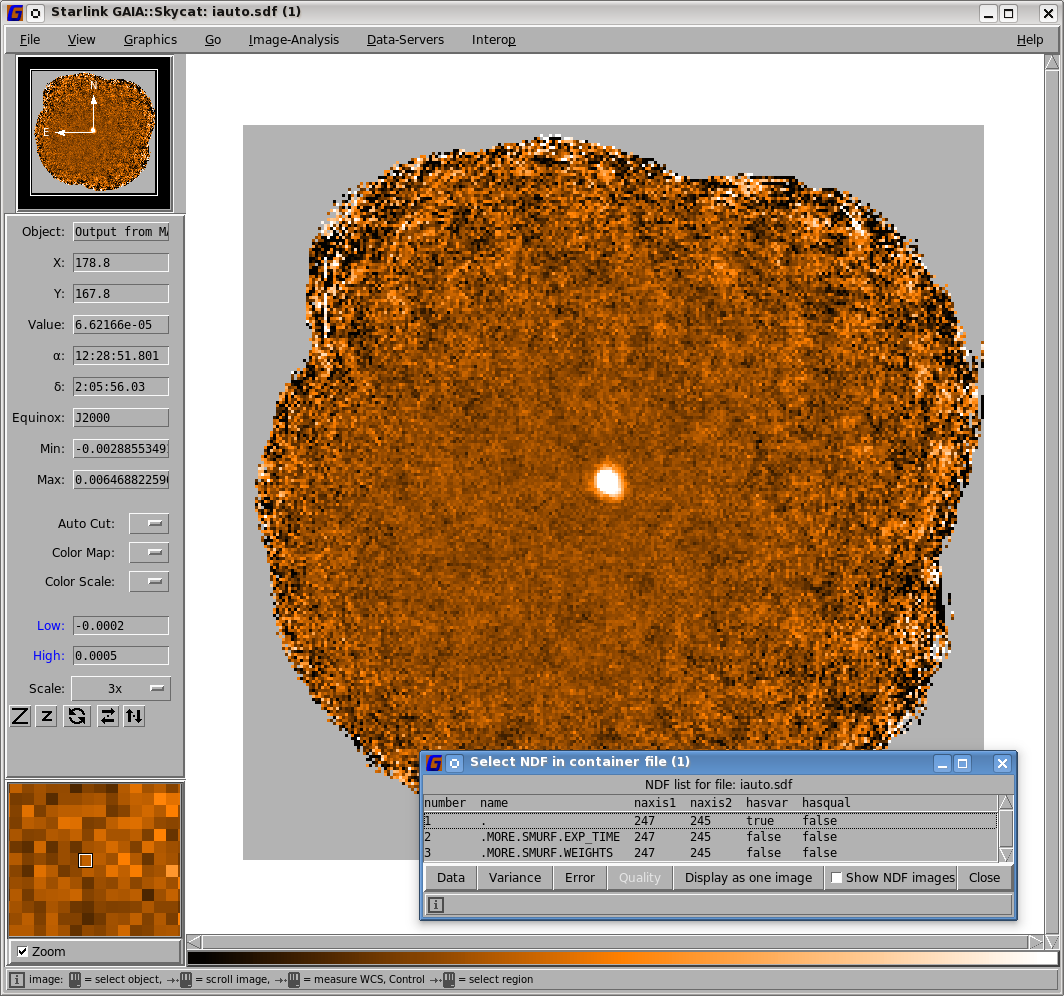
\includegraphics[width=0.8\linewidth]{sc22-gaia-view-iauto.png}
\label{fig:gaia-iauto}
\caption [I map in GAIA]{
  \small The I map, iauto.sdf, as viewed with GAIA. 
}
\end{center}
\end{figure}

The maps folder contains the individual I maps from each separate observation:

\begin{terminalv}
20160112_00056_0003_imap.sdf  20160112_00059_0003_imap.sdf  20160125_00043_0003_imap.sdf
\end{terminalv}

and the qudata folder contains:

\begin{terminalv}
s8a20160112_00056_0003_IT.sdf  s8b20160112_00059_0003_IT.sdf  s8c20160125_00043_0003_IT.sdf
s8a20160112_00056_0003_QT.sdf  s8b20160112_00059_0003_QT.sdf  s8c20160125_00043_0003_QT.sdf
s8a20160112_00056_0003_UT.sdf  s8b20160112_00059_0003_UT.sdf  s8c20160125_00043_0003_UT.sdf
s8a20160112_00059_0003_IT.sdf  s8b20160125_00043_0003_IT.sdf  s8d20160112_00056_0003_IT.sdf
s8a20160112_00059_0003_QT.sdf  s8b20160125_00043_0003_QT.sdf  s8d20160112_00056_0003_QT.sdf
s8a20160112_00059_0003_UT.sdf  s8b20160125_00043_0003_UT.sdf  s8d20160112_00056_0003_UT.sdf
s8a20160125_00043_0003_IT.sdf  s8c20160112_00056_0003_IT.sdf  s8d20160112_00059_0003_IT.sdf
s8a20160125_00043_0003_QT.sdf  s8c20160112_00056_0003_QT.sdf  s8d20160112_00059_0003_QT.sdf
s8a20160125_00043_0003_UT.sdf  s8c20160112_00056_0003_UT.sdf  s8d20160112_00059_0003_UT.sdf
s8b20160112_00056_0003_IT.sdf  s8c20160112_00059_0003_IT.sdf  s8d20160125_00043_0003_IT.sdf
s8b20160112_00056_0003_QT.sdf  s8c20160112_00059_0003_QT.sdf  s8d20160125_00043_0003_QT.sdf
s8b20160112_00056_0003_UT.sdf  s8c20160112_00059_0003_UT.sdf  s8d20160125_00043_0003_UT.sdf
\end{terminalv}


\section{\xlabel{how-step23}pol2map - producing the I, Q, U maps and catalogue}


As discussed in \cref{Chapter}{sec:dr}{POL-2 Data Reduction - The Theory} we need to take the I map output from the initial run of pol2map 
and use this to produce the final I, Q and U maps. If requested a vector catalogue is also produced.

The second and third steps of the POL-2 data reduction process,  can be run in a single command

\begin{terminalv}
% pol2map in=qudata/\* iout=iext qout=qext uout=uext mapdir=maps mask=iauto \
          maskout1=astmask maskout2=pcamask ipref=iext cat=mycat debias=yes
\end{terminalv}

The following shows the output from running this second pol2map command. First we see pol2map producing
new I maps for each map, correcting the position using from the intensity map provided by mask (in this case iauto.sdf)and then coadding all observations. 

\begin{terminalv}
Logging to file pol2map.log
(existing file pol2map.log moved to pol2map.log.1)

Masking will be based on SNR values in 'iauto'.

>>>>   Making I map from 20160112_00056_0003...

   Using pre-calculated pointing corrections of (1.889022181,2.8085505485) arc-seconds

>>>>   Making I map from 20160125_00043_0003...

   Using pre-calculated pointing corrections of (0.0,0.0) arc-seconds

>>>>   Making I map from 20160112_00059_0003...

   Using pre-calculated pointing corrections of (2.13319187001,2.40199783004) arc-seconds
Coadding I maps from all observations:
\end{terminalv}

we see as pol2map continues the Q and U maps are then produced, again with pointing corrections. This is followed by the creation of
the output vector catalogue:

\begin{terminalv}
>>>>   Making Q map from 20160112_00056_0003...

   Using pre-calculated pointing corrections of (1.889022181,2.8085505485) arc-seconds

>>>>   Making Q map from 20160125_00043_0003...

   Using pre-calculated pointing corrections of (0.0,0.0) arc-seconds

>>>>   Making Q map from 20160112_00059_0003...

   Using pre-calculated pointing corrections of (2.13319187001,2.40199783004) arc-seconds
Coadding Q maps from all observations:

>>>>   Making U map from 20160112_00056_0003...

   Using pre-calculated pointing corrections of (1.889022181,2.8085505485) arc-seconds

>>>>   Making U map from 20160125_00043_0003...

   Using pre-calculated pointing corrections of (0.0,0.0) arc-seconds

>>>>   Making U map from 20160112_00059_0003...

   Using pre-calculated pointing corrections of (2.13319187001,2.40199783004) arc-seconds
Coadding U maps from all observations:
Creating the output catalogue: 'mycat'...

45604 vectors written to the output catalogue.
\end{terminalv}


The output of this Final pol2map


\begin{terminalv}
astmask.sdf
pcamask.sdf
iext.sdf
qext.sdf
uext.sdf
mycat.FIT
\end{terminalv}


\begin{figure}[t!]
\begin{center}
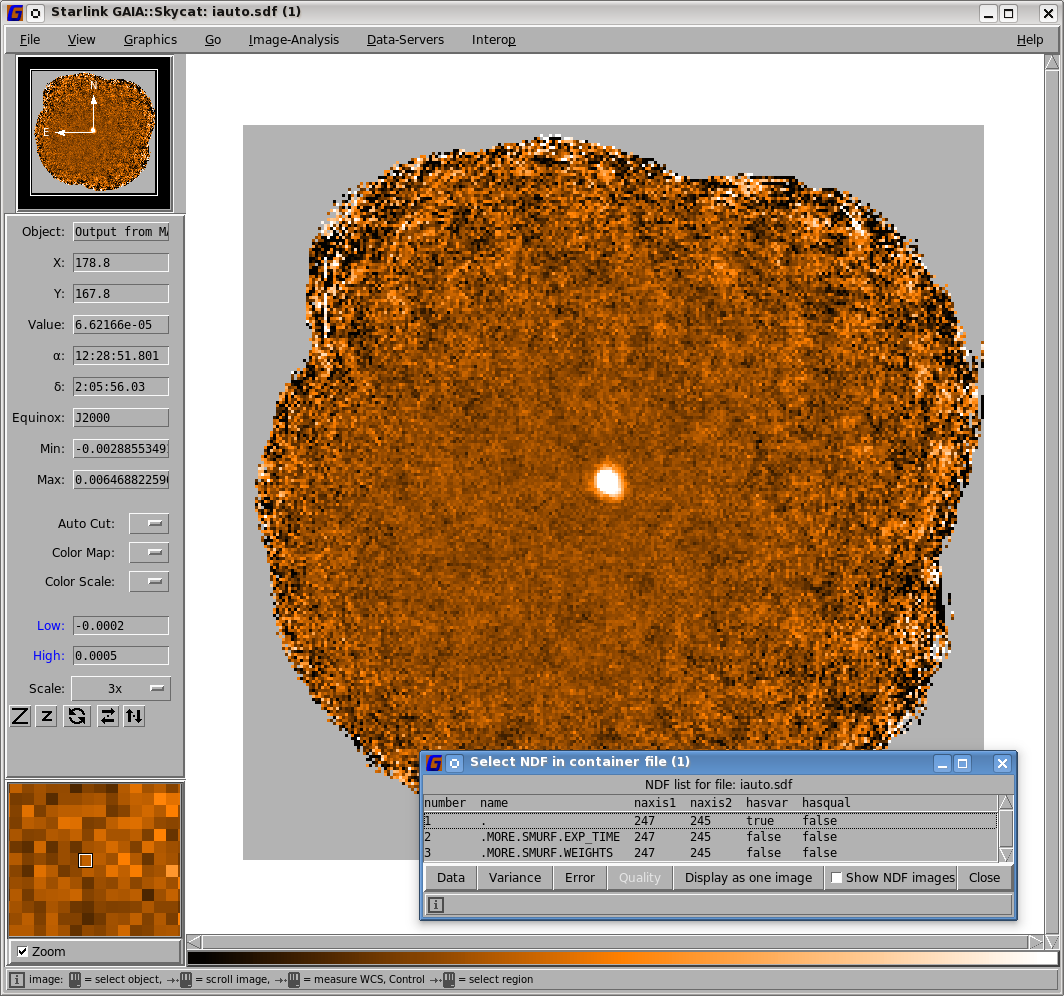
\includegraphics[width=0.46\linewidth]{sc22-gaia-view-iauto.png}
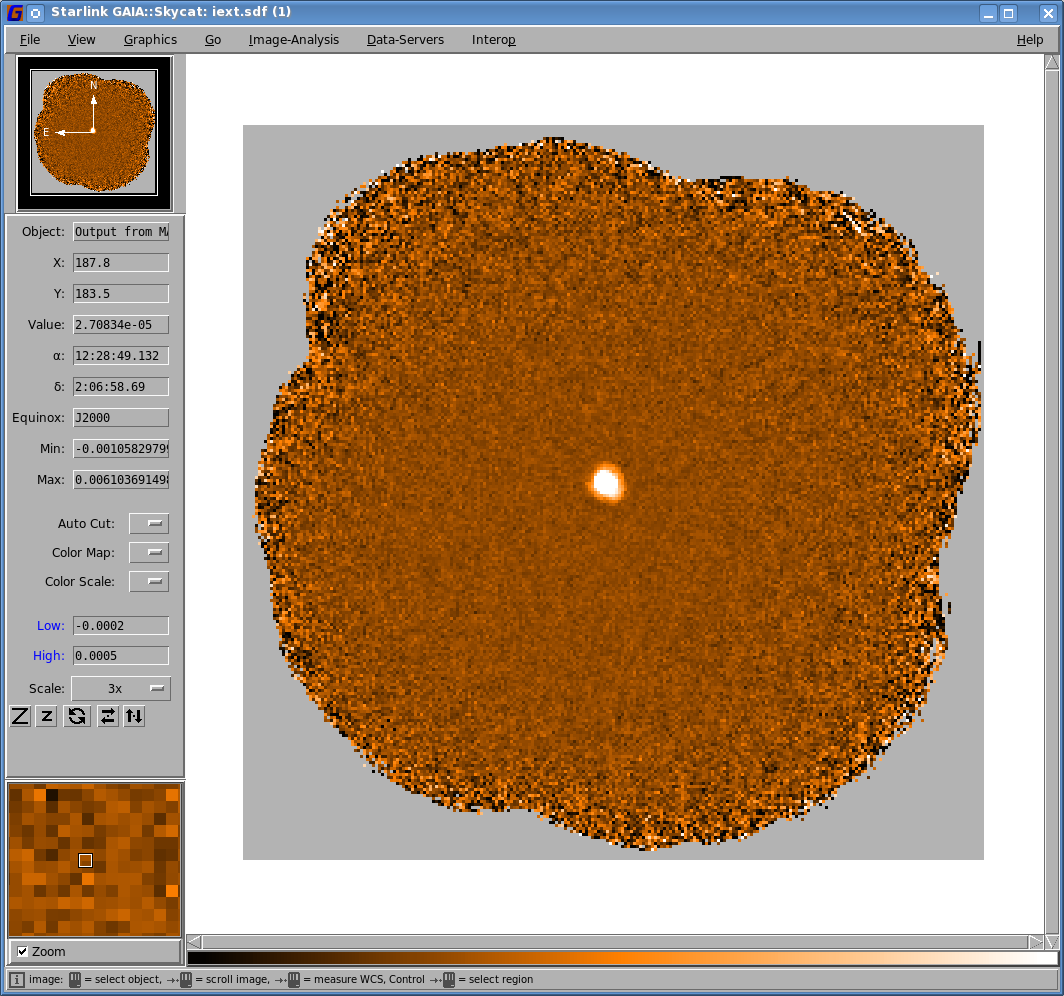
\includegraphics[width=0.46\linewidth]{sc22-gaia-view-iext.png}
\label{fig:gaia-iext}
\caption [Final I map in GAIA]{
  \small Left: I map, iauto, as produced by the automoask on the first pass of pol2map. Right: Final I map, iext, as viewed in GAIA.
}
\end{center}
\end{figure}


\begin{figure}[t!]
\begin{center}
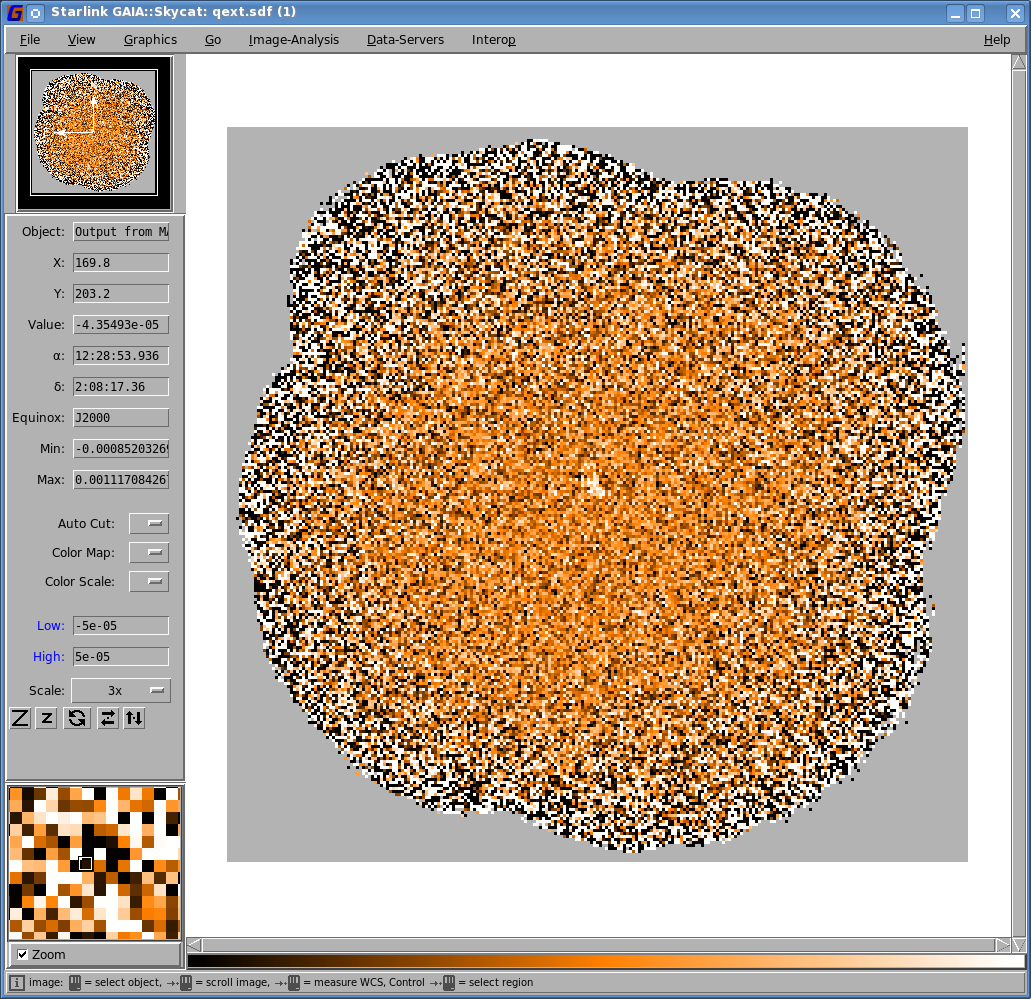
\includegraphics[width=0.46\linewidth]{sc22-gaia-view-qext.png}
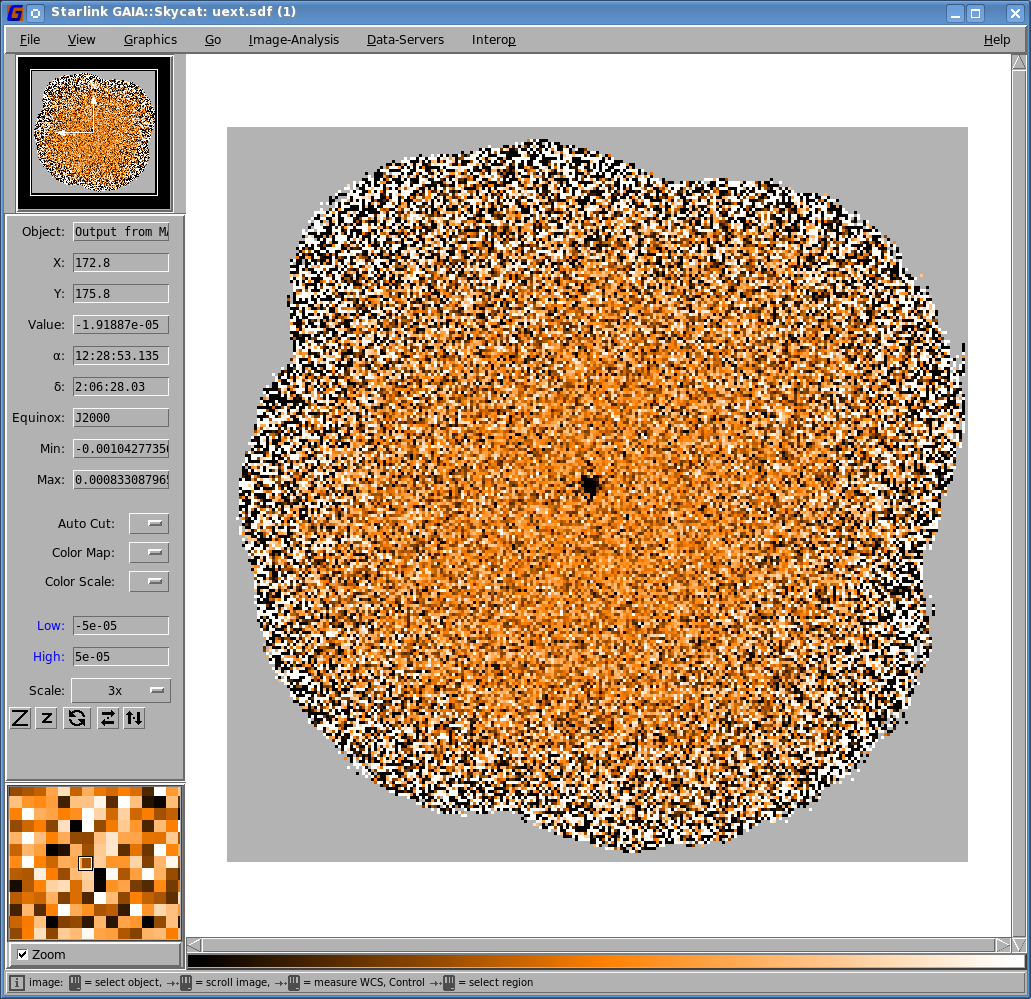
\includegraphics[width=0.46\linewidth]{sc22-gaia-view-uext.png}
\label{fig:gaia-qext-uext}
\caption [Q and U maps in GAIA]{
  \small Left: Q map, qext.sdf, Right: U map uext.sdf, as viewed with GAIA. 
}
\end{center}
\end{figure}



The maps folder now contains individual Q and U maps alongside the existing I maps:

\begin{terminalv}
20160112_00056_0003_Imap.sdf  20160112_00059_0003_Imap.sdf  20160125_00043_0003_Imap.sdf
20160112_00056_0003_Qmap.sdf  20160112_00059_0003_Qmap.sdf  20160125_00043_0003_Qmap.sdf
20160112_00056_0003_Umap.sdf  20160112_00059_0003_Umap.sdf  20160125_00043_0003_Umap.sdf
20160112_00056_0003_imap.sdf  20160112_00059_0003_imap.sdf  20160125_00043_0003_imap.sdf
\end{terminalv}




\section{\xlabel{vector-cat}Output vectors from pol2map}



The output vector catalogue, contains a range of values derived by pol2map for each pixel
contained within the I map. Values in the catalogue are in units of Jy/beam. 
The values are:

\begin{aligndesc}
\item[\texttt{X}] pixel coordinate
\item[\texttt{Y}] pixel coordinate
\item[\texttt{RA}] RA coordinate 
\item[\texttt{Dec}] Dec coordinate
\item[\texttt{I}] Intensity
\item[\texttt{DI}] error in I
\item[\texttt{Q}] stokes Q parameter
\item[\texttt{DQ}] error in Q
\item[\texttt{U}] stokes U parameter
\item[\texttt{DU}] error in U
\item[\texttt{P}] Percentage Polarization
\item[\texttt{DP}] error in P
\item[\texttt{ANG}] angle of polarization
\item[\texttt{DANG}] error in ANG
\item[\texttt{PI}] Polarized Intensity
\item[\texttt{DPI}] error in PI
\end{aligndesc}




\section{\xlabel{tweaking}Tweaking pol2map}
\label{sec:pol2map-tweaks}

Inevitably, as with SCUBA-2 data reduction, it will likely be necessary for a user to 
tweak the pol2map reduction for specific situations.

The pixel size of the final map produced is controlled by the pixsize
parameter in the the \smurf\ pol2map command:

\begin{terminalv}
% pol2map pixsize=12
\end{terminalv}



\section{\xlabel{config}The dimmconfig files for POL-2 reduction}
\label{sec:config}

When pol2map is run the reduction relies on a set of parameters 

\subsection*{.dimmconfig\_pol2.lis}

not to be directly used (hence hidden) .dimmconfig\_pol2.lis

numiter = -5




\begin{terminalv}
#  Use PCA to model and remove the  background polarisation.
   modelorder = (pca,ext,ast,noi)

#  Time based despiking.
   spikebox = 10
   spikethresh = 5

#  POL" scans are very slow, so avoid flagging slow samples.
   flagslow = 0.01

#  Aggreive noise clipping.
   noisecliphigh = 3

#  The data has already been downsampled by CALCQU, so don't  do any more
#  down sampling.
   downsampscale = 0

#  Weight bolometers using the RMS residuals calculated by CALQU and
#  stored i nthe variance component of the CALCQU output NDFs.
   noi.usevar = 1

#  Use smaller boxes when finding DC steps because of the very low sample
#  rate of POL2 Stokes vector time-series created by calcqu.
   dcfitbox = 5
   dcsmooth = 10
\end{terminalv}


\subsection*{dimmconfig\_pol2\_compact.lis}

This reduction builds on the default dimmconfig\_pol2.lis configuration file but uses boundary 
constraints for an initial ast mask since the source is assumed to be isolated.


\begin{terminalv}
   ast.zero_circle = (0.016666)
\end{terminalv}


\subsection*{dimmconfig\_pol2\_extended.lis}


This reduction builds on the default dimmconfig\_pol2.lis configuration file but

\begin{terminalv}
   numiter=-40
   ast.zero_snr = 3
   ast.zero_snrlo = 2
\end{terminalv}


 





